%% Ein einfaches Template für einen Übungsbericht unter Verwendung des Hagenberg
%% Setups, basierend auf der LaTeX 'report' Standardklasse.
%%% äöüÄÖÜß  <-- keine deutschen Umlaute hier? UTF-faehigen Editor verwenden!

%%% Magic Comments zum Setzen der korrekten Parameter in kompatiblen IDEs
% !TeX encoding = utf8
% !TeX program = pdflatex
% !TeX spellcheck = de_DE
% !BIB program = biber

\documentclass[german,notitlepage,smartquotes]{hgbreport}
% Zulässige Optionen in [..]:
%    Hauptsprache: 'german' (default), 'english'
%    Option zur Umwandlung in typografische Anführungszeichen: 'smartquotes'
%    APA Zitierstil: 'apa'
%    Erzeuge keine separate Titelseite: 'notitlepage'
%%%-----------------------------------------------------------------------------

\RequirePackage[utf8]{inputenc} % bei Verw. von lualatex oder xelatex entfernen!

\renewcommand{\chapter}[1]{} % Deaktiviere den \chapter Befehl
\graphicspath{{images/}}     % Verzeichnis mit Bildern und Grafiken
\bibliography{references}    % Biblatex-Literaturdatei (references.bib)
\ExecuteBibliographyOptions{backref=false} % Keine Rückreferenzen bei Quellen

%%%-----------------------------------------------------------------------------
\setcounter{chapter}{3}	% <----- Auf die Übungsnummer setzen
%%%-----------------------------------------------------------------------------

\author{Julian Jany}                        % Name
\title{BVA2 Fortgeschrittene Bildverarbeitung und -analyse -- SS 2022\\ % Name der Übung
				Übungsabgabe \arabic{chapter}}
\date{\today}

%%%-----------------------------------------------------------------------------
\begin{document}
%%%-----------------------------------------------------------------------------
\maketitle
%%%-----------------------------------------------------------------------------

%\begin{abstract}\noindent
%\ldots
%\end{abstract}

%%%-----------------------------------------------------------------------------

\section{Richardson Lucy Deconvolution}

\subsection{Problembeschreibung}

Es soll ein \texttt{ImageJ Plugin} entwickelt werden. 
Das Plugin soll den iterativen Algorithmus \textit{Richardson Lucy Deconvolution} anwenden, und damit ein \zB unscharfes Bild "scharfstellen" können. 

\subsection{Lösungsbeschreibung}

\subsection{Implementierung}

Hier werden interessante Code-Teile der Implementierung inkludiert.

\subsubsection{Extraktion der Buchstaben}

\subsection{Tests}

\subsubsection{Identische Kernel und kein Rauschen}

\begin{figure}[h]
	\centering\small
	\begin{tabular}{cc}
		\multicolumn{2}{c}{\FramePic{\includegraphics[width=0.7\textwidth]{ex-01-bridge-input}}} \\
		\multicolumn{2}{c}{(a)} \\
		\FramePic{\includegraphics[width=0.45\textwidth]{ex-01-bridge-blurred}} &
		\FramePic{\includegraphics[width=0.45\textwidth]{ex-01-bridge-rld-result}} \\
		(b) & (c)
	\end{tabular}
	\caption{Eingabe-Bild~(a); Gefiltertes Bild (Gauss; $\sigma=6.0$)~(b); Rekonstruiertes Bild~(c).}
	\label{fig:ex-01-bridge}
\end{figure}

\begin{figure}[h]
	\centering\small
	\begin{tabular}{cc}
		\multicolumn{2}{c}{\FramePic{\includegraphics[width=0.7\textwidth]{ex-01-bridge-input}}} \\
		\multicolumn{2}{c}{(a)} \\
		\FramePic{\includegraphics[width=0.45\textwidth]{ex-02-bridge-blurred}} &
		\FramePic{\includegraphics[width=0.45\textwidth]{ex-02-bridge-rld-result}} \\
		(b) & (c)
	\end{tabular}
	\caption{Eingabe-Bild~(a); Gefiltertes Bild (Gauss; $\sigma=6.0$)~(b); Rekonstruiertes Bild~(c).}
	\label{fig:ex-02-bridge}
\end{figure}

\begin{figure}[h]
	\centering\small
	\begin{tabular}{cc}
		\multicolumn{2}{c}{\FramePic{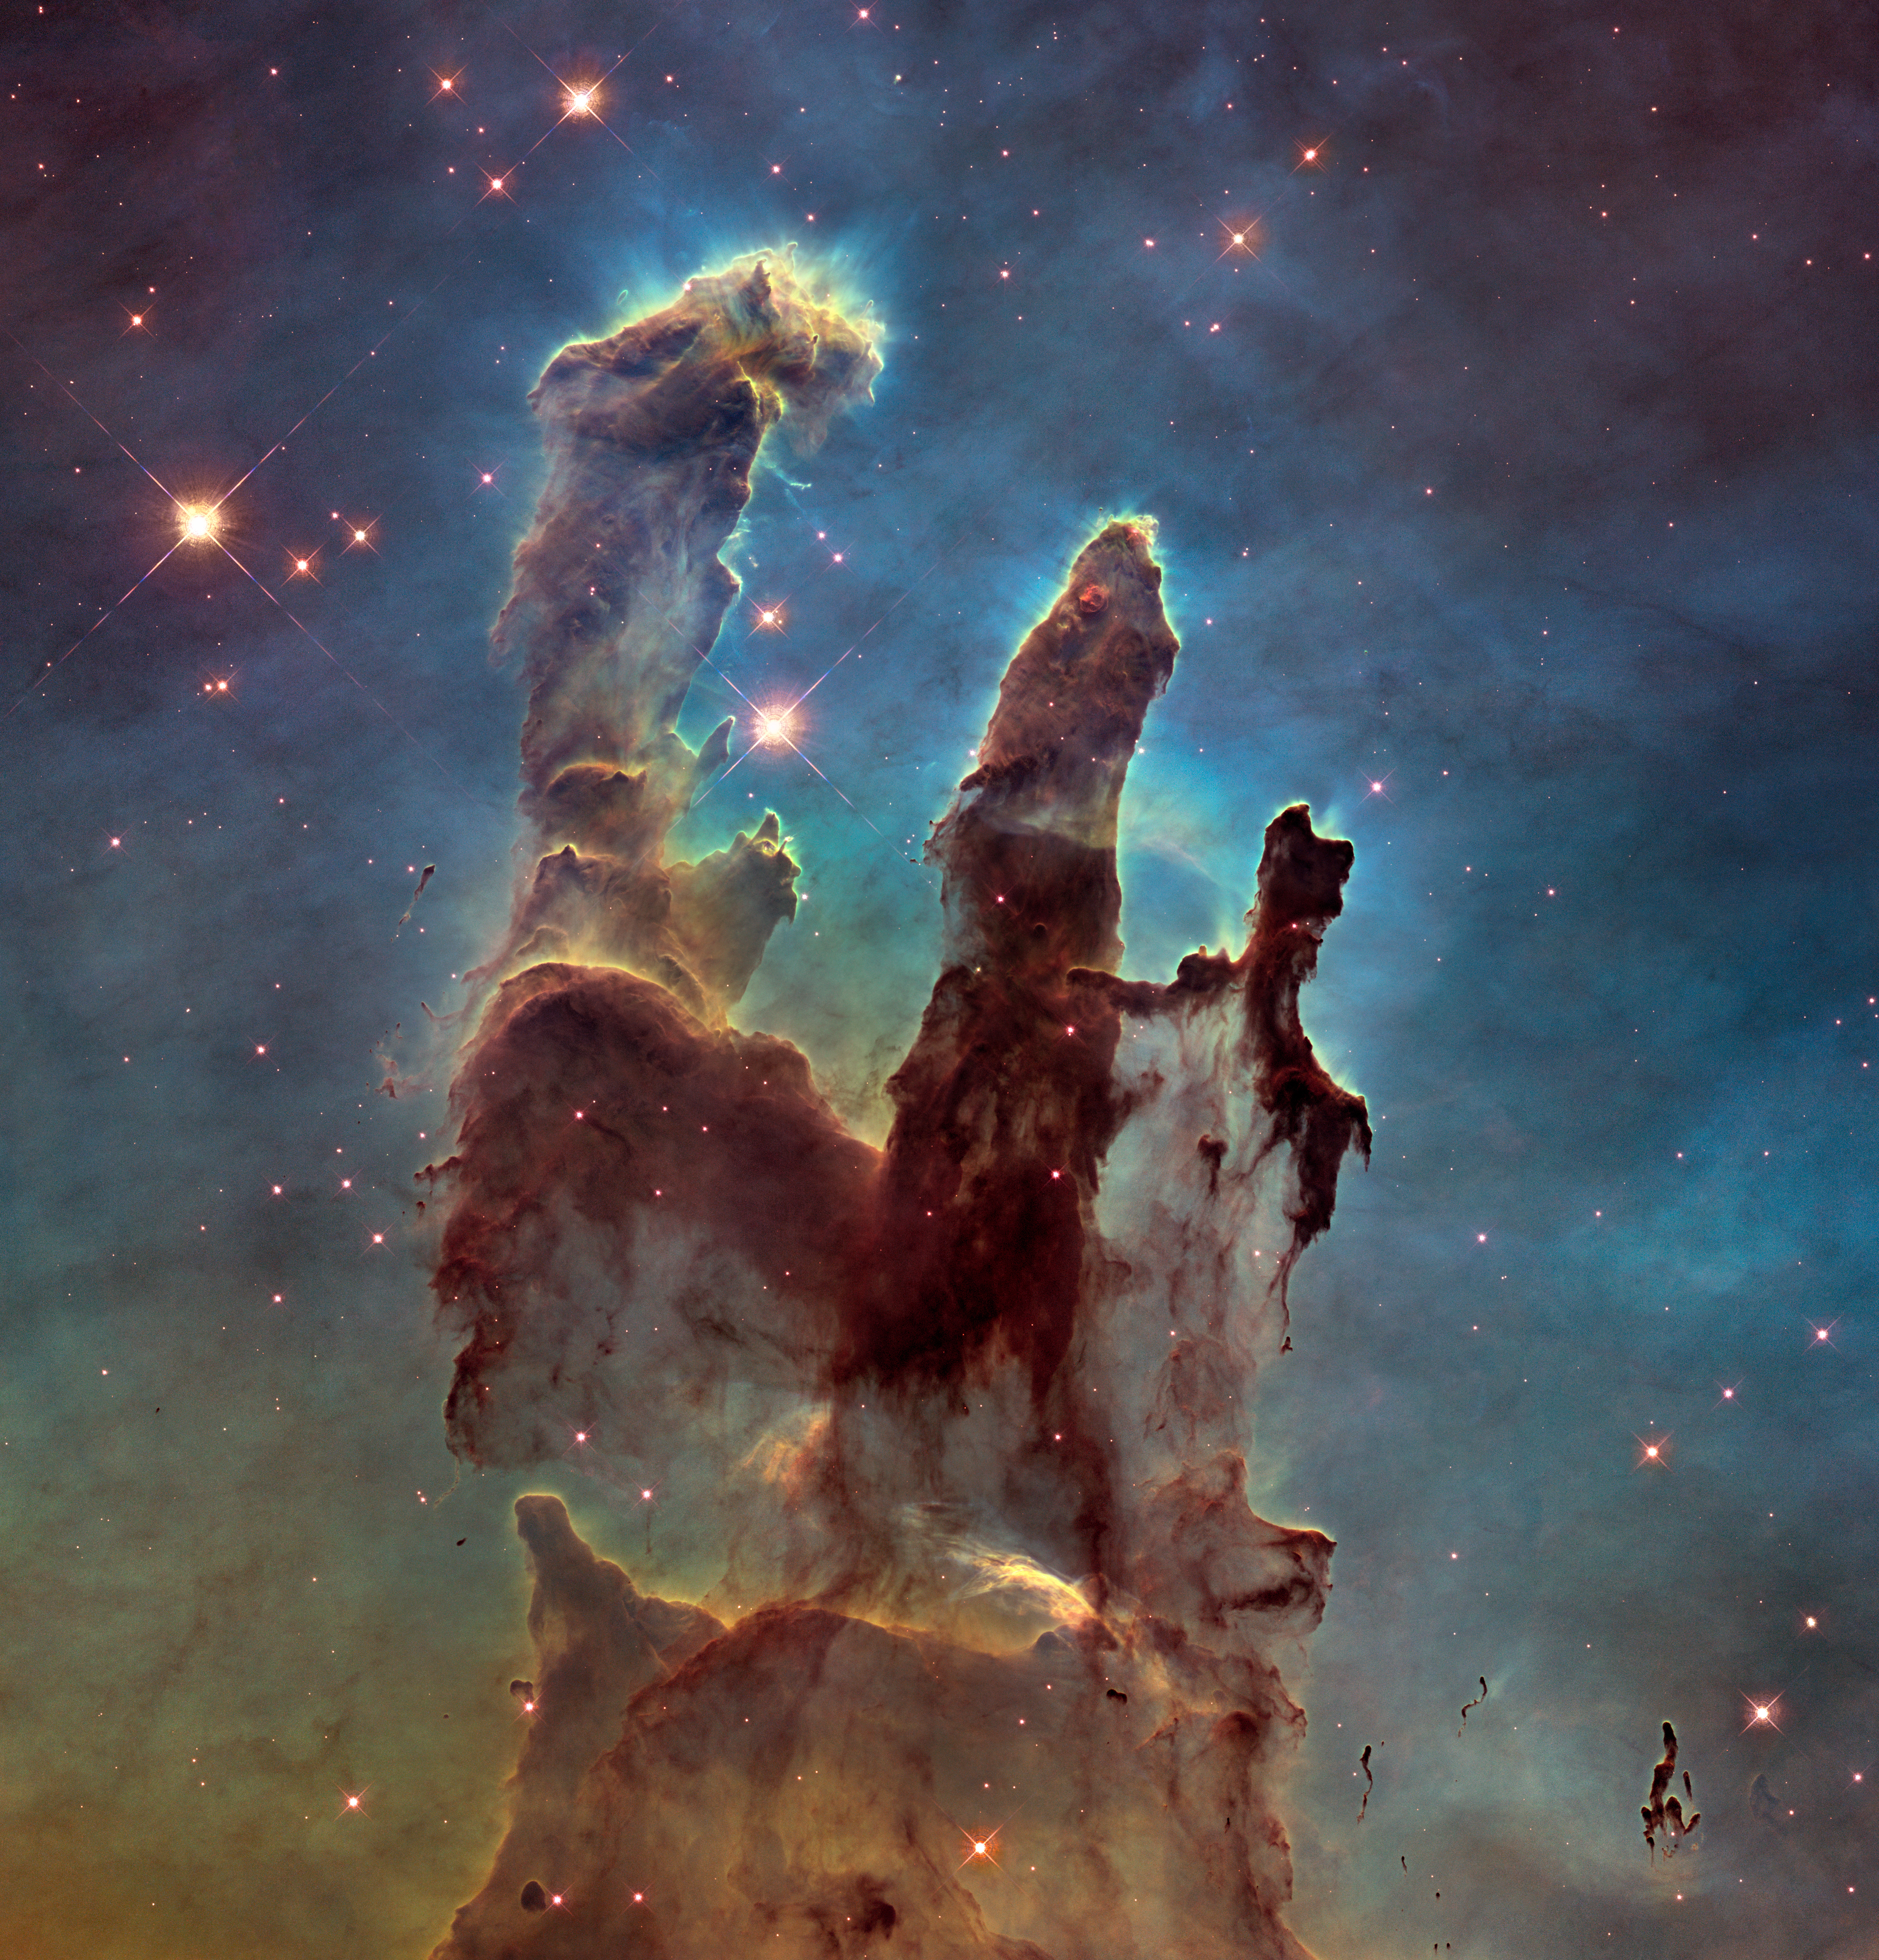
\includegraphics[width=0.7\textwidth]{heic1501a.jpg}}} \\
		\multicolumn{2}{c}{(a)} \\
		\FramePic{\includegraphics[width=0.45\textwidth]{ex-03-pillars-blurred}} &
		\FramePic{\includegraphics[width=0.45\textwidth]{ex-03-pillars-rld-result}} \\
		(b) & (c)
	\end{tabular}
	\caption{Eingabe-Bild~(a); Gefiltertes Bild (Gauss; $\sigma=6.0$)~(b); Rekonstruiertes Bild~(c).}
	\label{ex-03-pillars}
\end{figure}

\begin{figure}[h]
	\centering\small
	\begin{tabular}{cc}
		\multicolumn{2}{c}{\FramePic{\includegraphics[width=0.7\textwidth]{opo1000a.jpg}}} \\
		\multicolumn{2}{c}{(a)} \\
		\FramePic{\includegraphics[width=0.45\textwidth]{ex-04-galaxy-blurred}} &
		\FramePic{\includegraphics[width=0.45\textwidth]{ex-04-galaxy-rld-result}} \\
		(b) & (c)
	\end{tabular}
	\caption{Eingabe-Bild~(a); Gefiltertes Bild (Gauss; $\sigma=6.0$)~(b); Rekonstruiertes Bild~(c).}
	\label{ex-04-galaxy}
\end{figure}

\begin{figure}[h]
	\centering\small
	\begin{tabular}{cc}
		\multicolumn{2}{c}{\FramePic{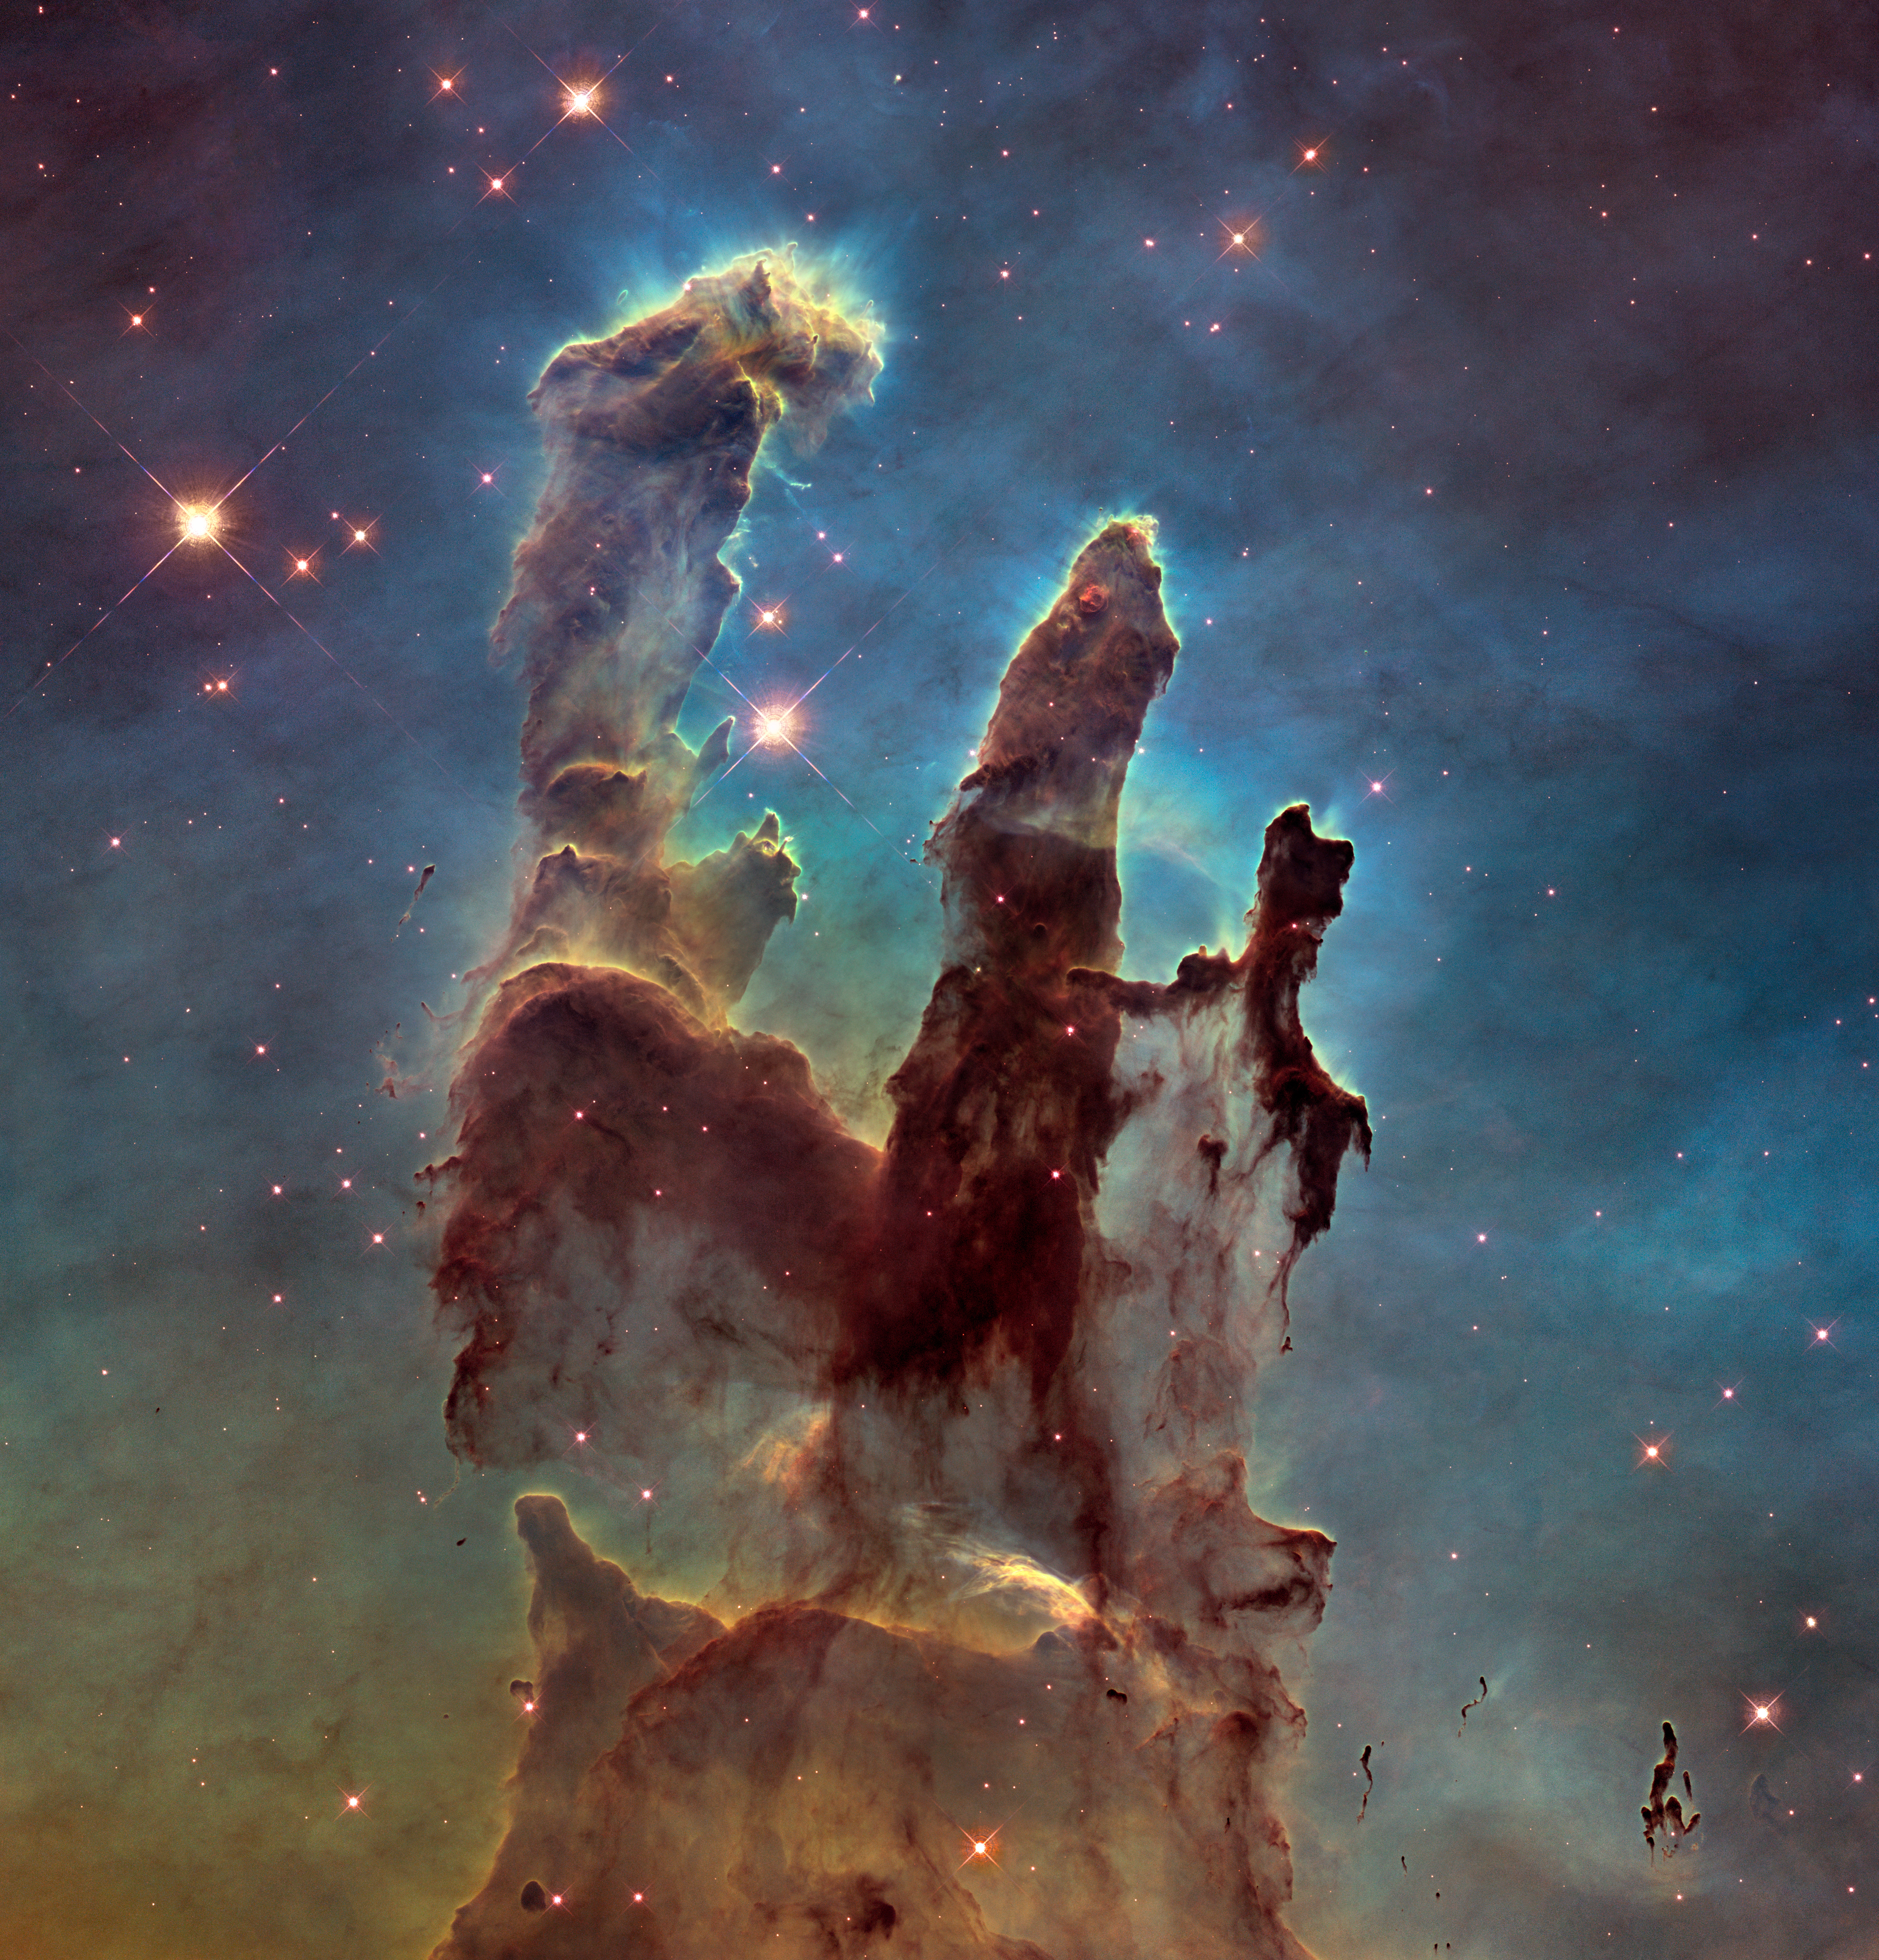
\includegraphics[width=0.7\textwidth]{heic1501a.jpg}}} \\
		\multicolumn{2}{c}{(a)} \\
		\FramePic{\includegraphics[width=0.45\textwidth]{ex-05-galaxy-blurred}} &
		\FramePic{\includegraphics[width=0.45\textwidth]{ex-05-galaxy-rld-result}} \\
		(b) & (c)
	\end{tabular}
	\caption{Eingabe-Bild~(a); Gefiltertes Bild (Gauss; $\sigma=6.0$)~(b); Rekonstruiertes Bild~(c).}
	\label{ex-05-galaxy}
\end{figure}

\begin{figure}[h]
	\centering\small
	\begin{tabular}{cc}
		\FramePic{\includegraphics[width=0.45\textwidth]{ex-04-galaxy-input}} &
		\FramePic{\includegraphics[width=0.45\textwidth]{ex-06-galaxy-rld-result-sharpened}} \\
		(a) & (b)
	\end{tabular}
	\caption{Eingabe-Bild~(a); Gefiltertes Bild (Gauss; $\sigma=6.0$)~(b); Rekonstruiertes Bild~(c).}
	\label{ex-06-galaxy}
\end{figure}

\begin{figure}[h]
	\centering\small
	\begin{tabular}{cc}
		% \multicolumn{2}{c}{\FramePic{\includegraphics[width=0.7\textwidth]{STScI-01EVVD1G3V0B3TY7J779XY5W1F.jpg}}} \\
		\multicolumn{2}{c}{(a)} \\
		\FramePic{\includegraphics[width=0.45\textwidth]{ex-07-deep-field-blurred}} &
		\FramePic{\includegraphics[width=0.45\textwidth]{ex-07-deep-field-rld-reconstructed}} \\
		(b) & (c)
	\end{tabular}
	\caption{Eingabe-Bild~(a); Gefiltertes Bild (Gauss; $\sigma=6.0$)~(b); Rekonstruiertes Bild~(c).}
	\label{ex-07-deep-field}
\end{figure}

% \begin{figure}[h]
% \centering
% \includegraphics[width=.7\textwidth]{test-01-A}
% \caption{Alle 'A' im Bild markiert.}
% \label{fig:test-01}
% \end{figure}


\subsection{Diskussion}

%%%-----------------------------------------------------------------------------

% \section{Titel der zweiten Aufgabe}

%%%-----------------------------------------------------------------------------

%\section*{Zusammenfassung und Anmerkungen}

%%%-----------------------------------------------------------------------------

% \section*{Quellen}

% \printbibliography[heading=noheader]

%%%-----------------------------------------------------------------------------
\end{document}
%%%-----------------------------------------------------------------------------